\graphicspath{{003L/input/}}


%Change defult figure nemas fom Figure 1 to Figure ###L-D1
\renewcommand{\thefigure}{003L-D\arabic{figure}}
%Figure 3
\begin{figure}[H]
	\centering
	\includegraphics[width=0.8\textwidth]{Fig1}
	\caption{Long-term study site 003L near Cathedral Wash.  (A), Map showing surveyed area.  Shown are locations of monumented control points, remote camera, and the computational boundary (blue dashed line).  Aerial imagery collected in May 2013 at a steady discharge of 227 m3/s.  (B) 1 meter DEM derived from the March 28, 2008, survey of combined ground and bathymetric point data.  Shown on the sandbar are the water-surface elevations reached by discharges of 227 and 708 m3/s (red and yellow lines, respectively).  Water-surface elevations are derived from relations provided in Appendix C.  Survey dates and geomorphic attributes are provided in Appendix A.  Flow is right to left in both A and B.  River mile is in GCMRC convention, with river mile 0 at Lees Ferry, Arizona.}
\end{figure}


% Figure 2
\begin{figure}[H]
	\centering
	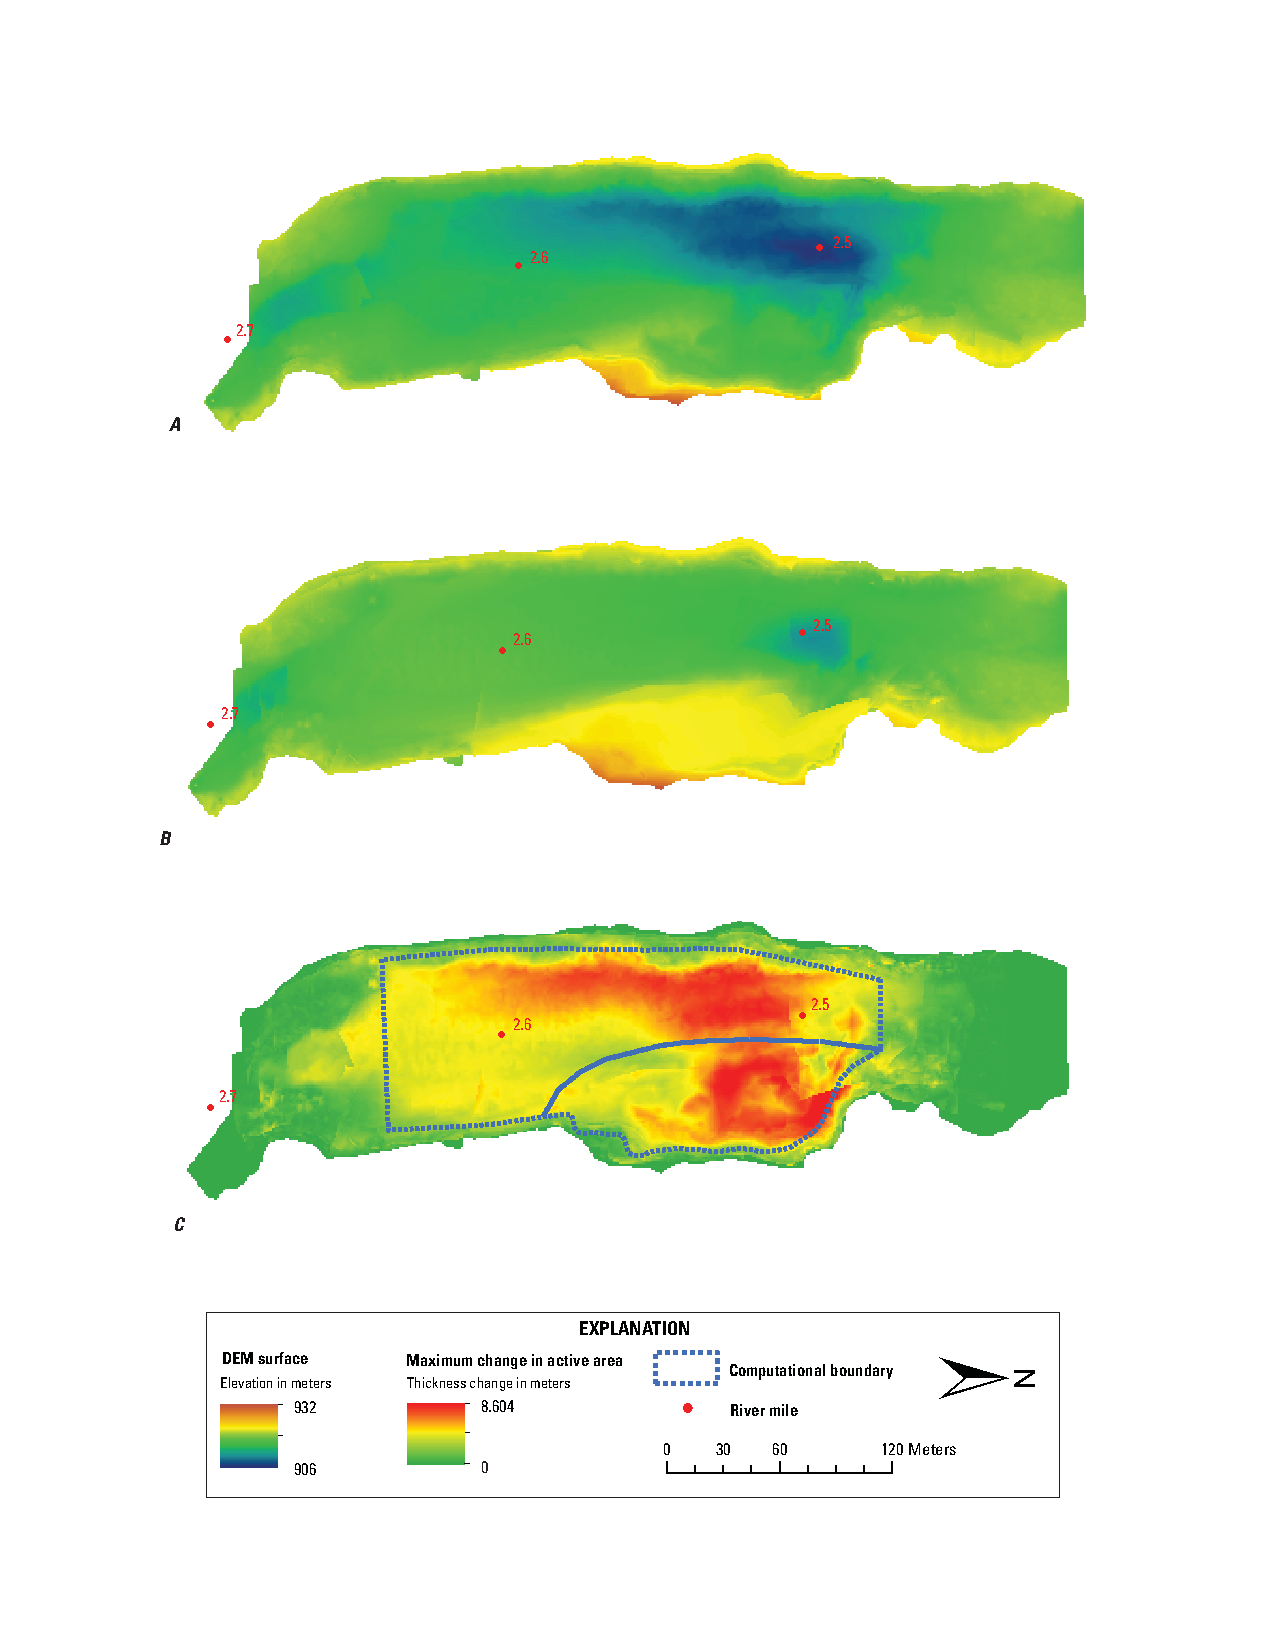
\includegraphics[width=0.8\textwidth]{Fig2}
	\caption{Long-term study site 003L near Cathedral Wash. Synthetic topography of the surveyed area in Fig. 003-D1 made by integrating the lowest and highest measured elevations collected since 1990 at 1-meter spaced grid nodes. (A) 1meter minimum surface DEM. (B) 1 meter maximum surface DEM. (C) Maximum potential active change based on subtracting the minimum (base level) surface from the maximum (potential) surface. The difference between these two surfaces is a conservative estimate of the maximum potential scour and fill, and thus of the active storage potential. The computational boundary is represented by the dashed blue line in C. Flow is right to left. River mile is in GCMRC convention, with river mile 0 at Lees Ferry, Arizona.}
\end{figure}


	%Figure 3
\begin{figure}[t!]
\centering
\subfigure[September 14, 1990]{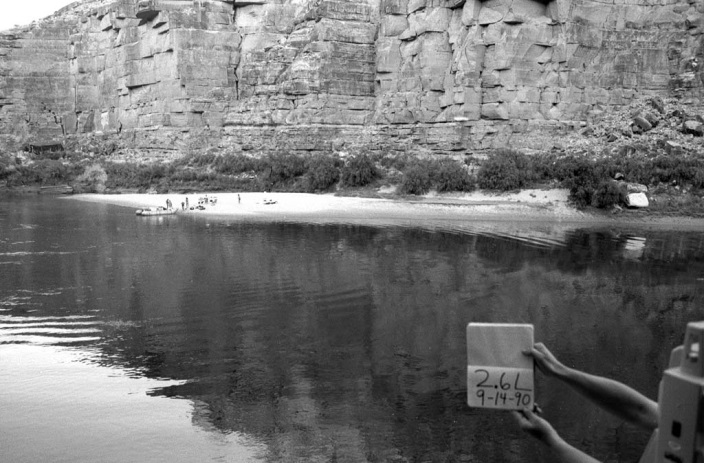
\includegraphics[width=3.2in]{image001}}
\subfigure[May 14, 1995]{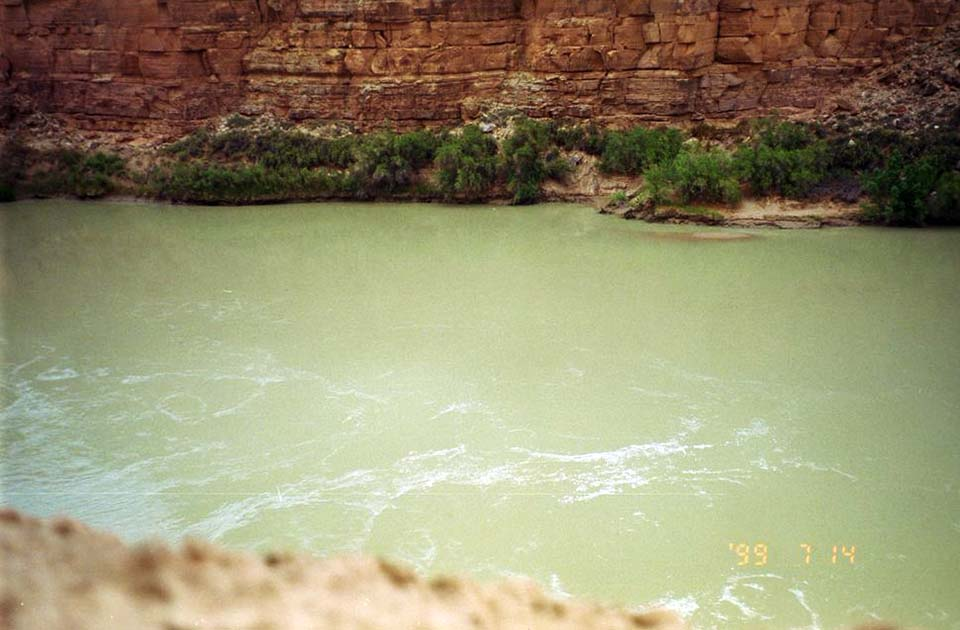
\includegraphics[width=3.2in]{image002}}
\subfigure[July 14, 1999]{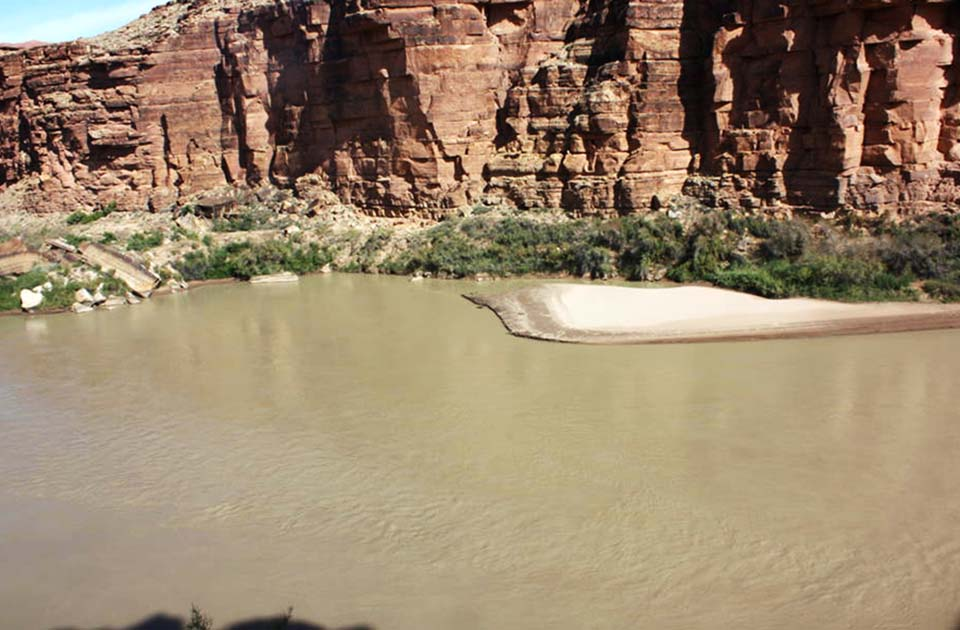
\includegraphics[width=3.2in]{image003}}
\subfigure[January 16, 2005]{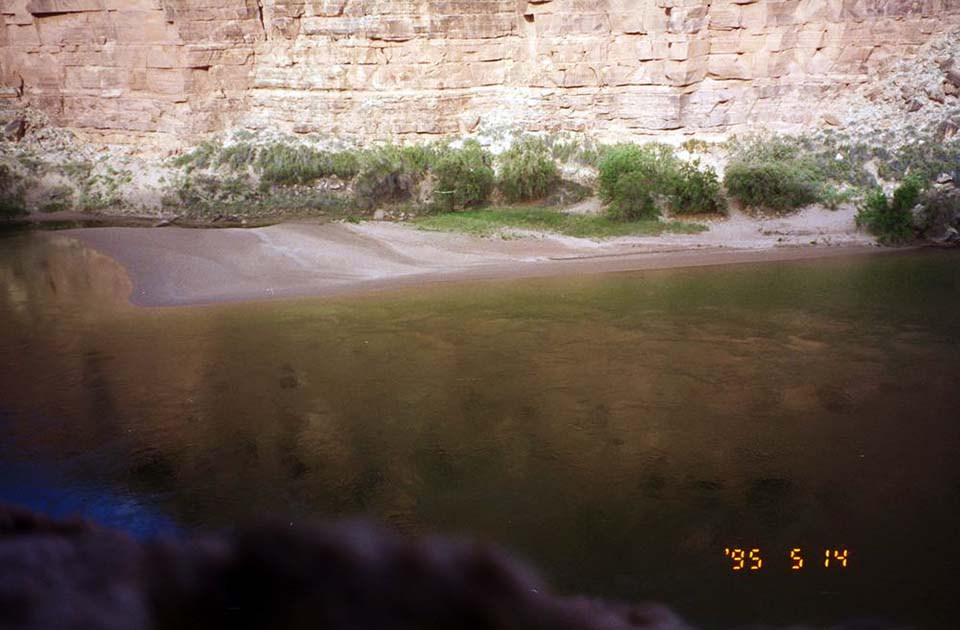
\includegraphics[width=3.2in]{image004}}
\subfigure[October 9, 2010]{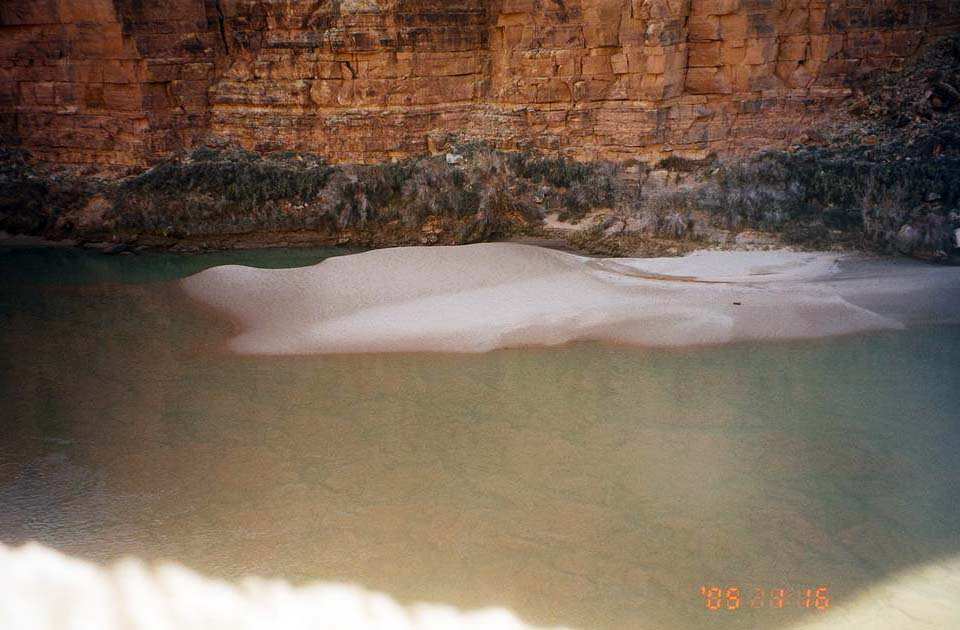
\includegraphics[width=3.2in]{image005}}
\subfigure[October 10, 2014]{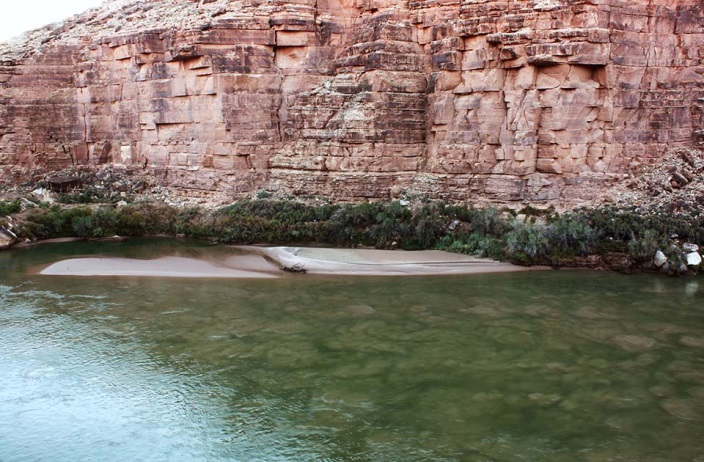
\includegraphics[width=3.2in]{image006}}
\caption{.  Selected photographs of long-term study site 003L near Cathedral Wash.  View is from the right bank of the river and shows the reattachment bar at various times between 1990 and 2014. Streamflow is from left to right.   }
\end{figure}
%Table1

\pgfplotstableset{
	begin table=\begin{longtable},
		end table=\end{longtable},
}
\newpage
\begin{landscape}
\begin{table}[H]
	\begin{center}
		\pgfplotstabletypeset[col sep=&, header=false, row sep=\\,
		every head row/.style={output empty row,
			before row={
				\toprule
				& \multicolumn{2}{c}{High Elevation} & \multicolumn{2}{c}{Fluctuating Zone}& \multicolumn{2}{c}{Low Elevation}& {Total Eddy} & {Total Channel} & {Total Site} \\
				\cmidrule(r){2-3} \cmidrule(r){4-5} \cmidrule(r){6-7} 
				{Survey Date}& {Area (m{$^2$})}  &{Volume (m{$^3$})}&{Area (m{$^2$})}&{Volume (m{$^3$})}&{Area (m{$^2$})}&{Volume (m{$^3$})} &{Volume (m{$^3$})}&{Volume (m{$^3$})}&{Volume (m{$^3$})}\\
				\midrule}},
		columns/0/.style={string type},
		columns/1/.style={string type},
		columns/2/.style={string type},
		columns/3/.style={string type},
		columns/4/.style={string type},
		columns/5/.style={string type},
		columns/6/.style={string type},
		columns/7/.style={string type},
		columns/8/.style={string type},
		columns/9/.style={string type}    
		]{
			4-7-1994&265&{$142   \pm  11$}&2,476&{$2,326  \pm 99$}&4,604&{$23,301  \pm 829$}&{$25,769  \pm 938$}&{$46,569  \pm 2,891$}&{$72,338  \pm 3,829$}\\
			4-7-1994&265&{$142   \pm  11$}&2,476&{$2,326  \pm 99$}&4,604&{$23,301  \pm 829$}&{$25,769  \pm 938$}&{$46,569  \pm 2,891$}&{$72,338  \pm 3,829$}\\}
	\end{center}
	
\end{table}

\end{landscape}
